\documentclass[../main.tex]{subfiles}
    \usepackage{amsmath}
    \usepackage{amsfonts}
    \usepackage{listings}
    \usepackage{graphicx}
    \graphicspath{ {img/} }

\begin{document}
\begin{enumerate}
	\item Wie viele Relationen auf einer endlichen Menge \( A \) mit \( n \) Elementen gibt es?

	      Lösung:
	      \begin{enumerate}
		      \item
	      \end{enumerate}
	\item Gib für \( A = \{x, y, z\} \) Relationen an mit folgenden Eigenschaften:
	      \begin{enumerate}
		      \item Reflexiv, aber nicht symmetrisch
		      \item Weder symmetrisch noch antisymmetrisch
		      \item Antisymmetrisch, aber nicht asymmetrisch
		      \item Total, aber nicht transitiv
		      \item Symmetrisch und total
	      \end{enumerate}

	      Lösung:
	      \begin{enumerate}
		      \item
	      \end{enumerate}
	\item Hier sind alle Relationen auf der Menge \( A = \{ x, y \} \):

	% 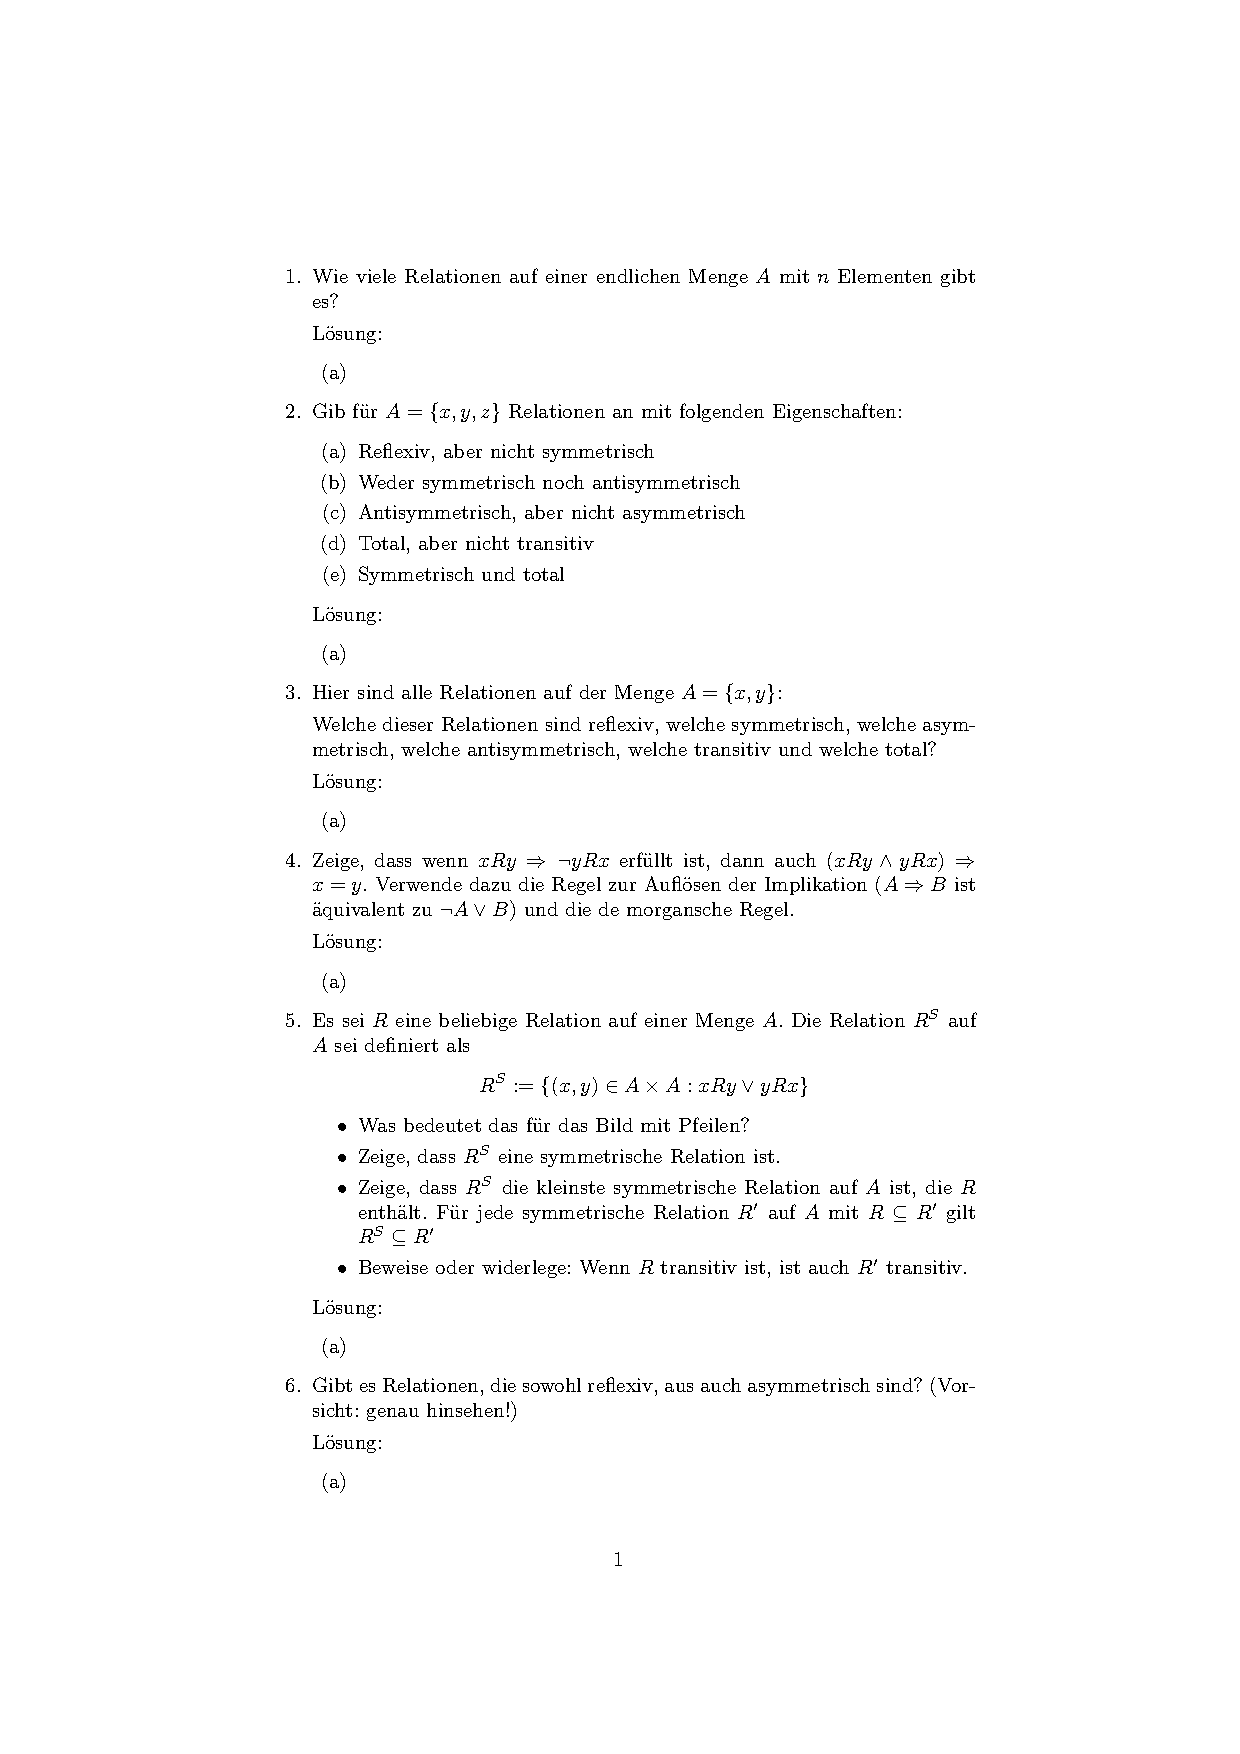
\includegraphics[scale=0.25]{relationen}

	      Welche dieser Relationen sind reflexiv, welche symmetrisch, welche asymmetrisch,
	      welche antisymmetrisch, welche transitiv und welche total?

	      Lösung:
	      \begin{enumerate}
		      \item
	      \end{enumerate}
	\item
	      Zeige, dass wenn \( xRy \Rightarrow \neg yRx \) erfüllt ist, dann auch
	      \( (xRy \land yRx) \Rightarrow x = y \).
	      Verwende dazu die Regel zur Auflösen der Implikation (\( A \Rightarrow B  \) ist äquivalent
	      zu \( \neg A \lor B \)) und die de morgansche Regel.

	      Lösung:
	      \begin{enumerate}
		      \item
	      \end{enumerate}
	\item Es sei \( R \) eine beliebige Relation auf einer Menge \( A \).
	      Die Relation \( R^S \) auf \( A \) sei definiert als
	      \[ R^S := \{ (x,y) \in A \times A : xRy \lor yRx \} \]
	      \begin{itemize}
		      \item Was bedeutet das für das Bild mit Pfeilen?
		      \item Zeige, dass \( R^S \) eine symmetrische Relation ist.
		      \item Zeige, dass \( R^S \) die kleinste symmetrische Relation auf \( A \) ist,
		            die \( R \) enthält.
		            Für jede symmetrische Relation \( R' \) auf \( A \) mit \( R \subseteq R' \)  gilt
		            \( R^S \subseteq R' \)
		      \item Beweise oder widerlege: Wenn \( R \) transitiv ist, ist auch \( R' \) transitiv.
	      \end{itemize}

		Lösung:
	      \begin{enumerate}
		      \item
	      \end{enumerate}
	\item Gibt es Relationen, die sowohl reflexiv, aus auch asymmetrisch sind?
	      (Vorsicht: genau hinsehen!)

	      Lösung:
	      \begin{enumerate}
		      \item
	      \end{enumerate}
\end{enumerate}
\end{document}